\documentclass{article}
%\usepackage{tgadventor}
%\renewcommand*\familydefault{\sfdefault} %% Only if the base font of the document is to be sans serif
%\usepackage[T1]{fontenc}

\usepackage[default]{comfortaa}
\usepackage{graphicx}
\usepackage{geometry}
\usepackage[T1]{fontenc}

\begin{document}
    \begin{titlepage}
        \title{Where should a board game caf\'{e} be located in Turku?}
        \author{Tom Bullock}
        \date{}
        \maketitle
        \thispagestyle{empty}
    \end{titlepage}

    \abstract{
        This report aims to answer the question "which districts in the city of Turku would be best suited for a board game caf\'e?" 
        As a city with a high number of board game players, and the nearest board game caf\'es being over two hours travel away, there is a noticeable gap in the market, and finding the right spot would prove incredibly lucrative.
        This question was answered by studying venue features within the vicinity of board game caf\'es around Europe, as well as the centres of major cities that do not possess them, and using these to train a logistic regression model to help calculate the suitability for districts of Turku.
        The resulting model was then used to determine the feasibility of each district of Turku, with these feasibilities visualised by a choropleth map. 
    }

    \newpage

    \tableofcontents

    \newpage

    \section{Introduction}

    sefoinsefi

    \section{Methodology}

    pkpoinuin

    \section{Results}

    gsgsopaopwmfd

    \begin{figure}[t]
        \centering
        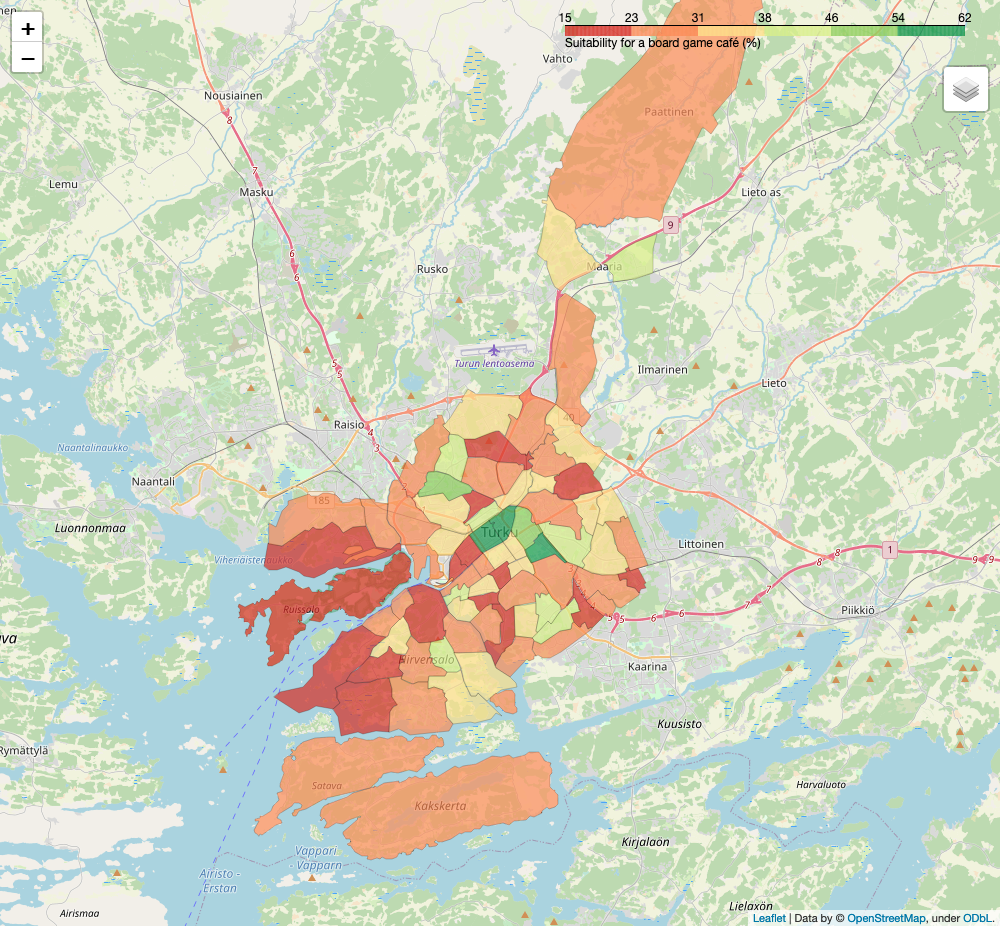
\includegraphics[width=0.8\textwidth]{Turku_map.png}
        \caption{\label{fig:Turkuprobs}The feasibility of each district of Turku. 
        Red and yellow regions would not make suitable candidates, whereas those in darker shades of green would be worth considering.}
    \end{figure}

    \section{Discussion}

    \section{Conclusions}


\end{document}